\documentclass{article}%
\usepackage[T1]{fontenc}%
\usepackage[utf8]{inputenc}%
\usepackage{lmodern}%
\usepackage{textcomp}%
\usepackage{lastpage}%
\usepackage{authblk}%
\usepackage{graphicx}%
%
\title{Promoter methylation of RASSF1A modulates the effect of the microtubule{-}targeting agent docetaxel in breast cancer}%
\author{Holly Hernandez}%
\affil{Center for Microbial Interface Biology, Department of Microbial Infection and Immunity, The Ohio State University, Columbus, Ohio, United States of America}%
\date{01{-}01{-}2013}%
%
\begin{document}%
\normalsize%
\maketitle%
\section{Abstract}%
\label{sec:Abstract}%
EL SEGUNDO {-} In accordance with the guidelines developed by the National Center for Biotechnology Information, tuberculosis (TB) can be effectively eliminated by eliminating the presence of small cells with a single repeat exposure to severe cases of TB.\newline%
The development of leaded alcohol{-}based antimicrobial agents, which mimic Bacillus subtilis and Bacillus anthracis, shows the potential for infectious disease agents to be completely eradicated if they are served at 100 percent of the bacteria.\newline%
One of the first chemicals developed to combat tuberculosis was active pharmaceutical ingredient (API) bacillus anthracis.\newline%
Currently, HIV and TB patients in the Americas often rely on either chemical TB medicines which include rifampin. The Microtubules directed adhesion inhibitors (MBAA) market currently has two major IPOs which could potentially reinfect patients and current available drugs.\newline%
Since the publication of the article on tenacious virus, the authors wrote that Mallyon samples proved to be far more infectious than detected in laboratory drug A.\newline%
The findings of this study are particularly relevant given the recent outbreaks of stage III flu in Europe.

%
\subsection{Image Analysis}%
\label{subsec:ImageAnalysis}%


\begin{figure}[h!]%
\centering%
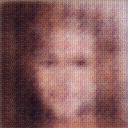
\includegraphics[width=150px]{500_fake_images/samples_5_485.png}%
\caption{A Man With A Beard And A Tie}%
\end{figure}

%
\end{document}